\label{sec:bosquejoGeneral}

\section{Arquitectura general}

	Con base en la teoría general de los sistemas según Ludwig von Bertalanffy, el sistema TLAMATINIME está conformado por dos sistemas. A continuación se detallan estos sistemas:
	
	\begin{itemize}
		\item \textbf{Sistema de Gestión de Información (SGI)}: Es el sistema encargado de gestionar la información requerida por el siguiente sistema.
				
		\item \textbf{Sistema de Soporte a las Decisiones (DSS)}: Este sistema muestra los resultados del algoritmo permitiendo al responsable tomar la decisión de utilizar esta opción de horario o generar una nueva.
	\end{itemize}
	
	En la figura~\ref{fig:sistemaT} se muestra la estructura de los sistemas que conforman al sistema en conjunto.

	\begin{figure}[htbp!]
		\begin{center}
			\fbox{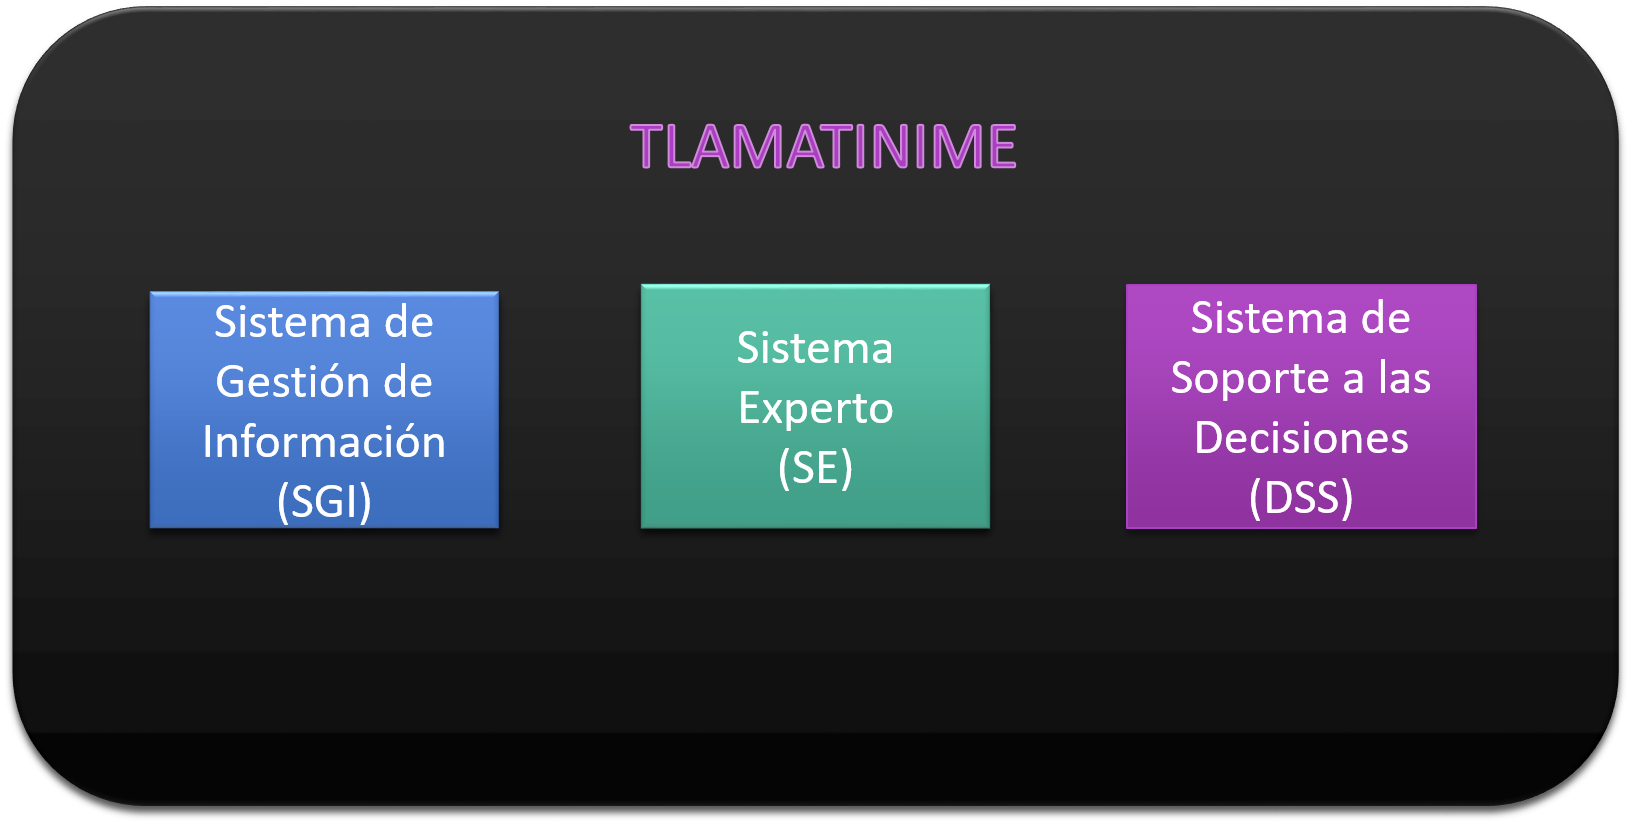
\includegraphics[width=.7\textwidth]{images/entornoTT/TLAMATINIME.png}}
			\caption{Modelo del sistema.}
			\label{fig:sistemaT}
		\end{center}
	\end{figure}

	

\section{Componentes}

	En la figura~\ref{fig:paquetes} se muestra el diagrama de paquetes que conforman el sistema.
	
	\begin{figure}[htbp!]
		\begin{center}
			\fbox{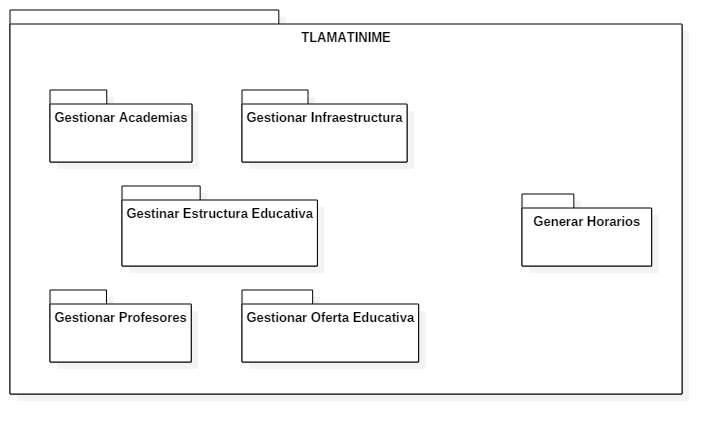
\includegraphics[width=.7\textwidth]{images/entornoTT/paquetes.png}}
			\caption{Diagrama de paquetes del sistema.}
			\label{fig:paquetes}
		\end{center}
	\end{figure}
	

\section{Requerimientos}

	Los requerimientos de un sistema de software son frecuentemente clasificados como requerimientos funcionales y requerimientos no funcionales: 

\subsection{Requerimientos funcionales}

	Estos son sentencias de los servicios que el sistema debería proporcionar, como el sistema debería reaccionar para entradas particulares, y como el sistema debería comportarse en situaciones particulares. En algunos casos, los requerimientos funcionales pueden decir explícitamente lo que el sistema no debe hacer. \\
	
	A continuación se enlistan los requerimientos funcionales identificados para el sistema.	
	
	\begin{itemize}
		\item El sistema debe permitir al subdirector académico seleccionar las unidades de aprendizaje que se impartirán durante un semestre.
		
		\item El sistema debe permitir al subdirector académico asignar a un profesor las unidades de aprendizaje que impartirá durante el semestre.
		
		\item El sistema debe permitir al subdirector académico consultar los horarios una vez generados.
		
		\item El sistema debe permitir al subdirector académico seleccionar un horario.
		
		\item El sistema debe permitir al subdirector académico realizar modificaciones al horario seleccionado.
		
		\item Un profesor tiene un número finito de unidades de aprendizaje que debe impartir al semestre.
		
		\item Un profesor no puede estar en dos clases al mismo tiempo.
		Las unidades de aprendizaje así como los grupos deben estar divididas por nivel.
		
		\item Las unidades teórico-prácticas tienen un espacio para sus clases de práctica.
		
		\item Una unidad de aprendizaje no puede ser impartida más de una vez en el mismo grupo.
		
		\item Se debe priorizar que los profesores tengan la carga que deberían tener.
		
	\end{itemize}
	

\subsection{Requerimientos no funcionales}
	
	Estas son restricciones en los servicios o funciones que ofrece el sistema. Estos incluyen restricciones de tiempo, restricciones del proceso de desarrollo, y restricciones impuestas por estándares. Estos frecuentemente aplican a los sistemas como un todo, en vez de aplicar a características o servicios individuales del sistema. \\
	
	A continuación se enlistan los requerimientos no funcionales con los que cumplirá el sistema.
	
	\subsubsection{Diseño}
	
	\begin{itemize}
		\item \textbf{LaTeX:} El documento en donde se concentrará todo el análisis de este trabajo será LaTeX, desarrollado por Leslie Lamport en 1984. LaTeX es multiplataforma y está orientado a la creación de documentos escritos, de modo que, estos  presentan una alta calidad tipográfica. La versión de LaTeX utilizada es LaTeX2e News Issue 27. [2]
		
		\item \textbf{Balsamiq Mockups:} Es una aplicación que facilita y agiliza la creación de bocetos. Esto nos permite crear las interfaces que muestran las gestiones del sistema. Balsamiq cuenta con una aplicación nativa para OS X (también Windows y Linux) y una versión web. La versión de Balsamiq Mockups utilizada es 3.5.15 para Windows. [3] [4]
		
		\item \textbf{StarUML:} Es una herramienta que permite modelar los estándares UML. StarUML nos permitirá diagramar los casos de uso y diagramas de paquetes del sistema. La versión de StarUML utilizada es 2.8.1 para Windows. [5]
		
		\item \textbf{HTML5:} (HyperText Markup Language) desarrollo a cargo del Consorcio W3C. El término representa dos conceptos diferentes: Se trata de una nueva versión de HTML, con nuevos elementos, atributos y comportamientos. Contiene un conjunto más amplio de tecnologías que permite a los sitios Web y a las aplicaciones ser más diversas y de gran alcance. [7]
		
		\item \textbf{CSS3:} Es la última evolución del lenguaje de las Hojas de Estilo en Cascada (Cascading Style Sheets). Trae consigo muchas novedades como las esquinas redondeadas, sombras, gradientes , transiciones o animaciones, y nuevos layouts como multi-columnas, cajas flexibles o maquetas de diseño en cuadrícula (grid layouts). [8]
		
		\item \textbf{JavaScript:} Es un lenguaje de programación interpretado, dialecto del estándar ECMAScript. Se utiliza principalmente en su forma del lado del cliente (client-side). Para interactuar con una página web se provee al lenguaje JavaScript de una implementación del Document Object Model (DOM). La versión de JS utilizada es ECMAScript 2016. [11]
				
		\item \textbf{Identidad gráfica:} En la figura~\ref{fig:entornoTrabajo} se muestra el entorno sobre el que se trabajan las pantallas del sistema, y a continuación se describe cada una se las secciones que la componen.
		
		\begin{figure}[htbp!]
			\begin{center}
				\fbox{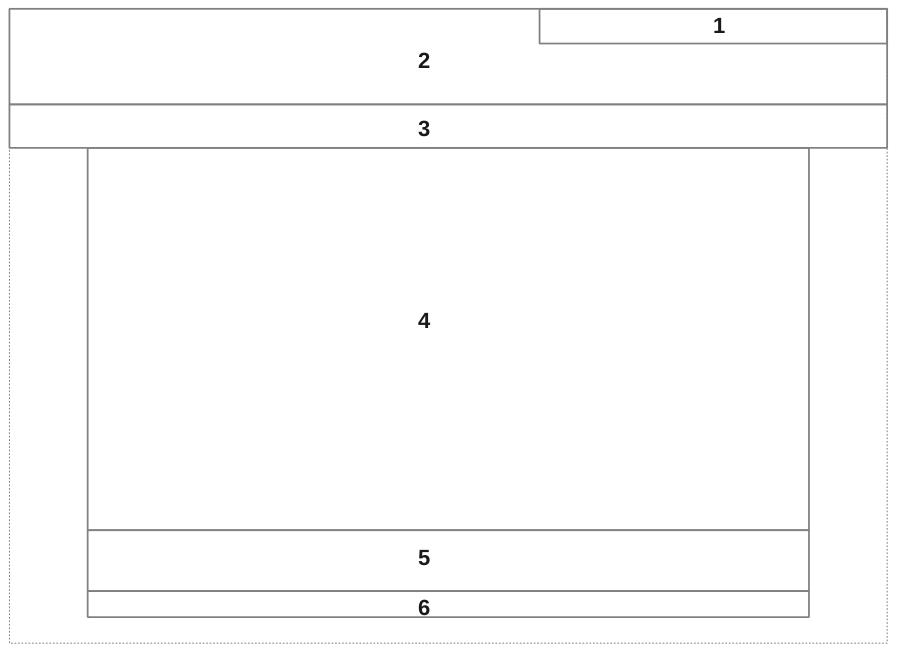
\includegraphics[width=.8\textwidth]{images/entornoTT/entornoTrabajo.png}}
				\caption{Entorno de trabajo del sistema}
				\label{fig:entornoTrabajo}
			\end{center}
		\end{figure}	
		
		\begin{itemize}
			\item Sección 1: se mostrará el usuario del actor que esté ingresando al sistema en ese momento.
			
			\item Sección 2: contiene el menú que nos permitirá navegar a través de la aplicación. Además, se mostrará el encabezado con los logos del IPN y de la ESCOM. 
			
			\item Sección 3: representa el área de trabajo, en esta se mostrarán las gestiones, formularios de registros, etc.
			
			\item Sección 4: se destina este espacio para el footer, el cual destacará todo aquello que en la página web haya podido pasar desapercibido.
		\end{itemize}
		
		
	\end{itemize}
	
	\subsubsection{Construcción}
	
	\begin{itemize}
		\item \textbf{Phyton:} En este lenguaje de programación diseñado por Guido Van Rossum en 1991, se desarrollará el algoritmo genético. Una de las ventajas que nos proporciona phyton es que es multiplataforma, es decir, puede implementarse e interoperar en múltiples plataformas. Se eligió este lenguaje debido a que es fácil aprenderlo y existe documentación que puede apoyar en este proceso. La versión de phyton utilizada es 3.5.0 [1] 
		
		A continuación se muestra una tabla en la que se agrupan las características, ventajas y desventajas de algunos lenguajes de programación.
		
		\resizebox*{16cm}{10cm}{
			\begin{tabular}{|l|l|l|l|}
				\hline
				Nombre & Características & Ventajas & Desventajas\\
				\hline
				
				RUBY & Orientado a objetos. &  Portátil  & Es relativamente nuevo y no cuenta\\
				
				&&&con mucha documentación. \\
				
				& Lenguaje de alto nivel. & Desarrollo de bajo costo. & No está muy difundido como otros \\
				
				&&& lenguajes.\\
				
				& Sintaxis similar a Python y Perl. & Multiplataforma & \\
				
				& Lenguaje para la creación de aplicaciones  & & \\
				
				& de escritorio y aplicaciones web. & & \\
				
				
				\hline
				ASP.NET & Creada por Microsoft. &  Controles de usuarios y personalizados.  & Alto consumo de recursos. \\
				
				& De paga & Fácil mantenimiento. & \\
				
				& Orientado a objetos. & Incremento en velocidad. & \\
				
				& & Mayor seguridad. & \\
				
				
				\hline
				Python & Permite la creación de todo tipo de  & Libre y código fuente abierto. & Al ser interpretado, puede presentar una  \\
				
				& programas incluso sitios web. && lentitud relativa.\\
				
				& No requiere de compilación es un código.  & Fácil mantenimiento. & Multiplataforma  \\
				
				& interpretado. && \\
				
				& Orientado a objetos. &  & \\
				
				& Portable & & \\
				
				& Simple, legible y similar al idioma inglés. & & \\
				
				
				\hline
				C++ & Orientado a objetos & Ideal para sistemas robustos & No soporta creación de aplicaciones web.\\
				
				& & IDEs de desarrollo son DEV C++, & Complejo visualmente. \\
				
				&& BORLAND C, TURBO C.&\\
				
				& & Multiplaforma & \\
				
				& & Rápido & \\
				
				
				\hline
				
				Java & Orientado a objetos. & Permite la creación de aplicaciones de & Al ser interpretado, puede presentar una  \\
				
				&& escritorio, móviles y web.& lentitud relativa. \\
				
				& Multiplataforma && \\
				
				
				\hline
		\end{tabular}}
		
		
		\item \textbf{Django:} Es un framework de desarrollo web que respeta el patrón de diseño conocido como Modelo–vista–template. Django pone énfasis en el re-uso, la conectividad y extensibilidad de componentes, el desarrollo rápido y el principio No te repitas (DRY, del inglés Don't Repeat Yourself) que promueve la reducción de la duplicación. La versión de django utilizada es 2.0.2 [6] \\
		
		En la figura~\ref{fig:django} se muestra la arquitectura utilizada por el framework Django.
		
		\begin{figure}[htbp!]
			\begin{center}
				\fbox{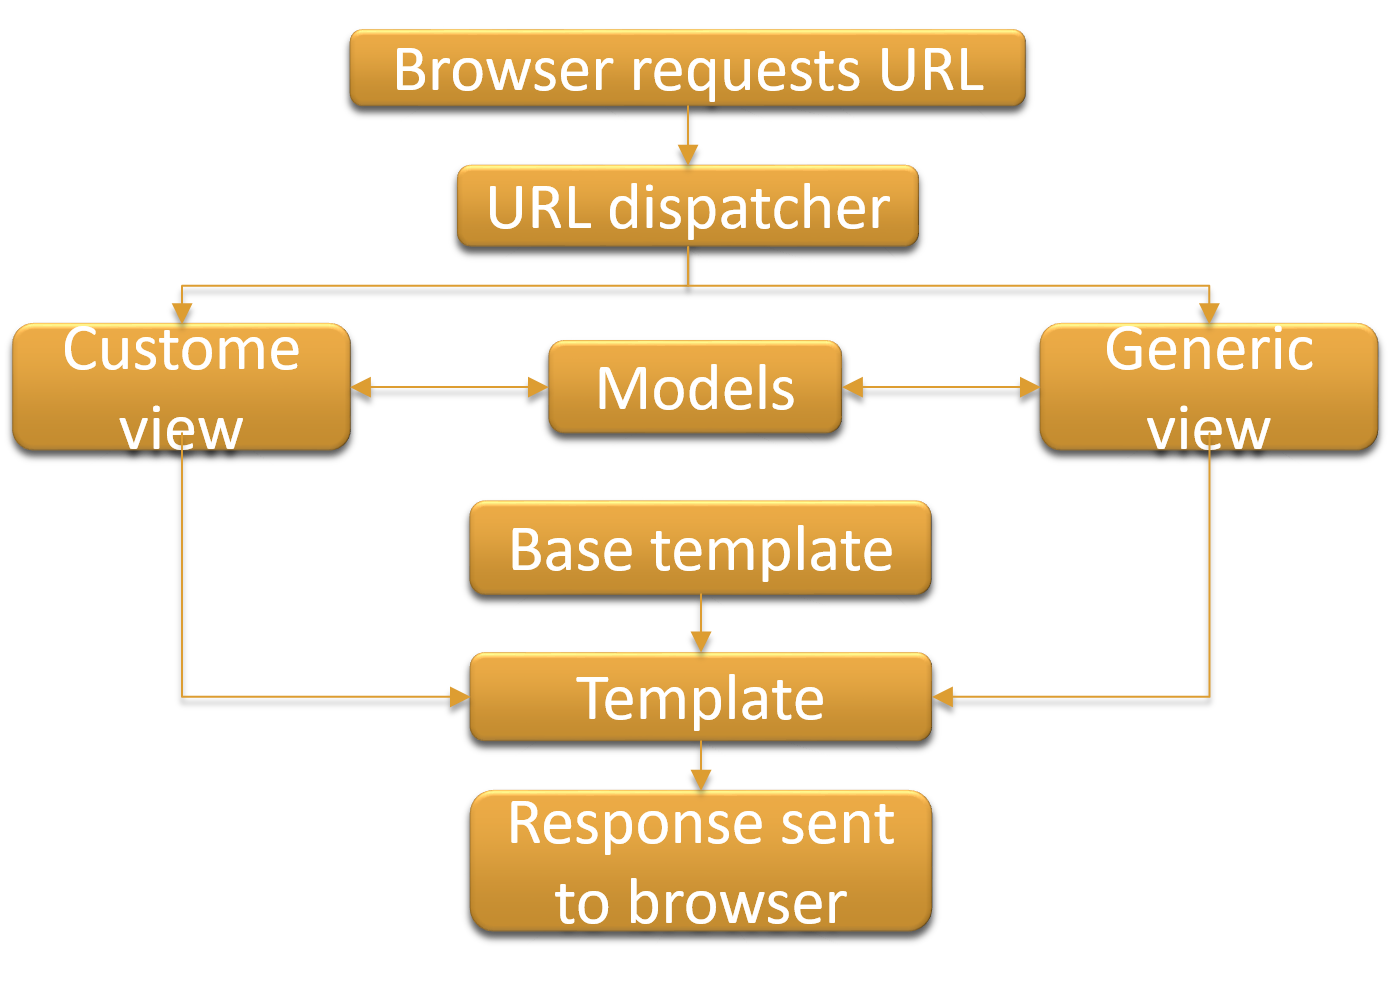
\includegraphics[width=.55\textwidth]{images/entornoTT/django.png}}
				\caption{Arquitectura Django}
				\label{fig:django}
			\end{center}
		\end{figure}
		
	\end{itemize}
	
	La aplicación ocupa el patrón MTV (Modelo-Platilla-Vista), a continuación de describe en que consiste.
	
	\begin{itemize}
		\item \textbf{Modelo:} Es la fuente única y definitiva de los datos de nuestra aplicación que nos permite realizar operaciones con ellos.
		Dicho de otra forma, un modelo se entiende como una tabla de la base de datos que soporta nuestra aplicación.
		El gran beneficio que tenemos es el ORM (Object-Relational mapping), es decir, el mapeo objeto–relacional, del cual ya no tendremos que ocuparnos.
		Todos nuestros modelos extienden (heredan) de la clase django.db.models.Model
		Los modelos tienen atributos que se convierten en campos en las tablas de la base de datos.
		
		\item \textbf{Vista:} Es el elemento de nuestra aplicación donde ponemos la lógica de negocio así como las funciones necesarias de apoyo.
		Aquí se procesan las peticiones o solicitudes (request) que accederán al Modelo para poder obtener o entregar datos.
		La vista genera una respuesta, para el caso de Django se utiliza el método render para establecer la plantilla (template) de destino hacia dónde irán los datos.
		Dicho de otra forma, aquí se establece la lógica necesaria para devolver una respuesta (y que datos conforma dicha respuesta) hacia el cliente que la solicita.
		
		\item \textbf{Plantilla:} Es el elemento (documento HTML) que decide CÓMO se van a mostrar los datos devueltos por la vista.
		Cada plantilla obtiene una respuesta proveniente de la vista correspondiente y contiene la estructura necesaria para presentar los datos en la forma necesaria utilizando estilos CSS o brindando dinamismo a través de JavaScript.
	\end{itemize}
	
	
	
		
	\subsubsection{Validación}
	
		\begin{itemize}
			
			\item \textbf{Navegadores:} Se han elegido los siguientes navegadores con base en la estadística tomada de StatCounter. [9] 
			
			\begin{figure}[htbp!]
				\begin{center}
					\fbox{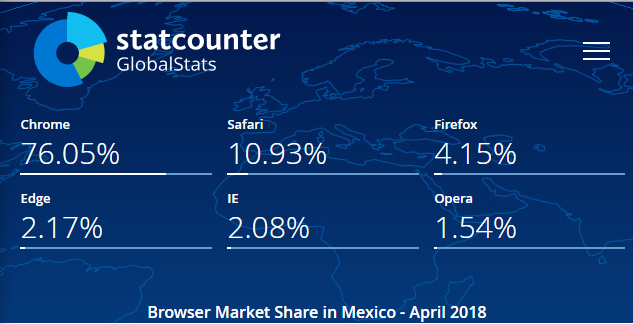
\includegraphics[width=.8\textwidth]{images/entornoTT/navegadores.png}}
					\caption{Estadística de los navegadores utilizados en México}
					\label{fig:navegadores}
				\end{center}
			\end{figure}
			
			En la figura~\ref{fig:navegadores} muestra que \textbf{Chrome} es el navegador más utilizado en México con un 76.05\% y se ha elegido por la popularidad que tiene. Por otro lado, se eligió como navegador alterno \textbf{IE} con una utilización del 2.08\%, aunque este no es el más utilizado es el navegador que viene instalado por defecto en Windows.
			
			\item \textbf{Sistema de servidores:} En la figura~\ref{fig:servidor} muestra la comunicación entre la interacción del cliente con el sistema alojado en el servidor y la base de datos.
			
			\begin{figure}[htbp!]
				\begin{center}
					\fbox{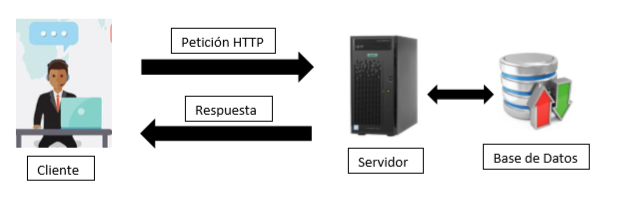
\includegraphics[width=.8\textwidth]{images/entornoTT/servidor.png}}
					\caption{Comunicación del sistema}
					\label{fig:servidor}
				\end{center}
			\end{figure}
			
			
			
			\item \textbf{Sistema operativo usuarios:} En la figura~\ref{fig:so} muestra que windows está posicionado como el sistema operativo más utilizado con un 81.73\%. Se elige windows 10 de 64 bits como sistema operativo en el que será instalado el sistema debido a la popularidad que tiene y que dentro de la ESCOM es utilizado en su mayoría por el personal administrativo, nuestro principal usuario.
			
			\begin{figure}[htbp!]
				\begin{center}
					\fbox{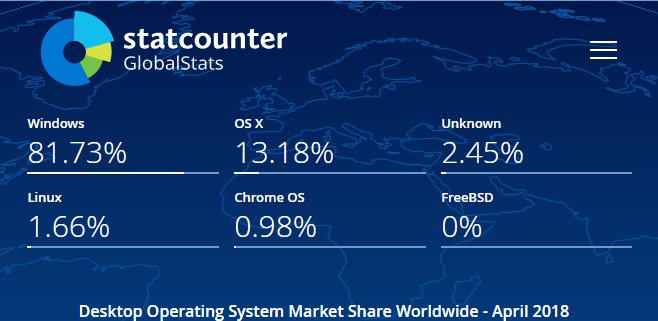
\includegraphics[width=.8\textwidth]{images/entornoTT/so.png}}
					\caption{Estadística de los sistemas operativos utilizados en México}
					\label{fig:so}
				\end{center}
			\end{figure}
		
			
		\end{itemize}
	
	\subsubsection{Propiedades no funcionales}
		\begin{itemize}
			\item \textbf{Complejidad:} Se define como el grado en que un sistema de software o uno de sus componentes ha sido diseñado o implementado de forma que es difícil de entender y verificar. Este requerimiento en particular se satisface dividiendo el sistemas en partes pequeñas que sean sencillas de entender.De igual manera eliminamos las dependencias innecesarias entre los componentes del sistema.
			En la figura~\ref{fig:vistalogica} muestra la forma en que se comunican los diferentes paquetes del sistema.
				
				\begin{figure}[htbp!]
					\begin{center}
						\fbox{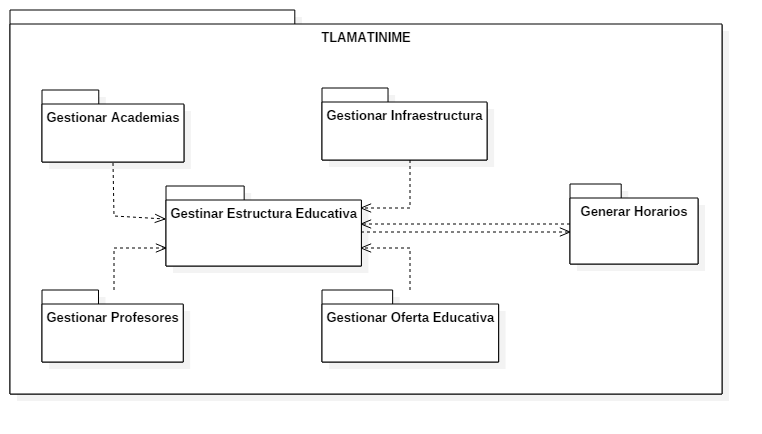
\includegraphics[width=.5\textwidth]{images/entornoTT/vistalogica.png}}
						\caption{Comunicación entre paquetes}
						\label{fig:vistalogica}
					\end{center}
				\end{figure}
			
			\item \textbf{Portabilidad:} Habilidad de un sistema de ser ejecutado en distintas plataformas con modificaciones mínimas sin conflictuar las características funcionales y no funcionales. El sistema diseñado y sus componentes deben ser portables en plataformas GNU/Linux y Windows, con máquinas que presentan arquitecturas de 64 bits. 
						
			\item \textbf{Escalabilidad:} Es la capacidad del sistema de ser adaptado para ajustarse a nuevos requerimientos. La escalabilidad no sólo cuida que el sistema pueda adaptarse a cambios en el alcance o en el tamaño, cuida también que pueda cambiar para ajustarse a nuevas funcionalidades solicitadas. Hace referencia a la capacidad del sistema de crecer sin desmejorar la calidad del servicio que presta. El diseño por módulos del sistema permite que sea escalable.
			
			\item \textbf{Documentación:} Se especificará el análisis y especificaciones de diseño en la documentación técnica, de modo que, esto permitirá que el sistema pueda ser mantenible.
			
			\item \textbf{Trazabilidad:} La información permite que se encuentren dependencias entre los requisitos y los componentes del diseño del
			sistema y la documentación. Así, la información permitirá evaluar los cambios de requerimientos.
		%	\item \textbf{Heterogeneidad}
		\end{itemize}
	
